\section{UML Activities and Surface Languages}
\label{sec:grammars-and-metamodels:Preliminaries}

The surface language we present is a textual alternative for the activity diagrams of the \UML.
In this section, we give a brief description of Activities and explain what a surface language is.
We use the naming convention used by the \OMG in the definition of the \UML~\cite{UMLsuper} when discussing concepts of the \UML.
This means that we use medial capitals for the names of these concepts.


\subsection{UML Activities}
\label{sub:grammars-and-metamodels:UML-Activities}

\begin{figure}
\centering
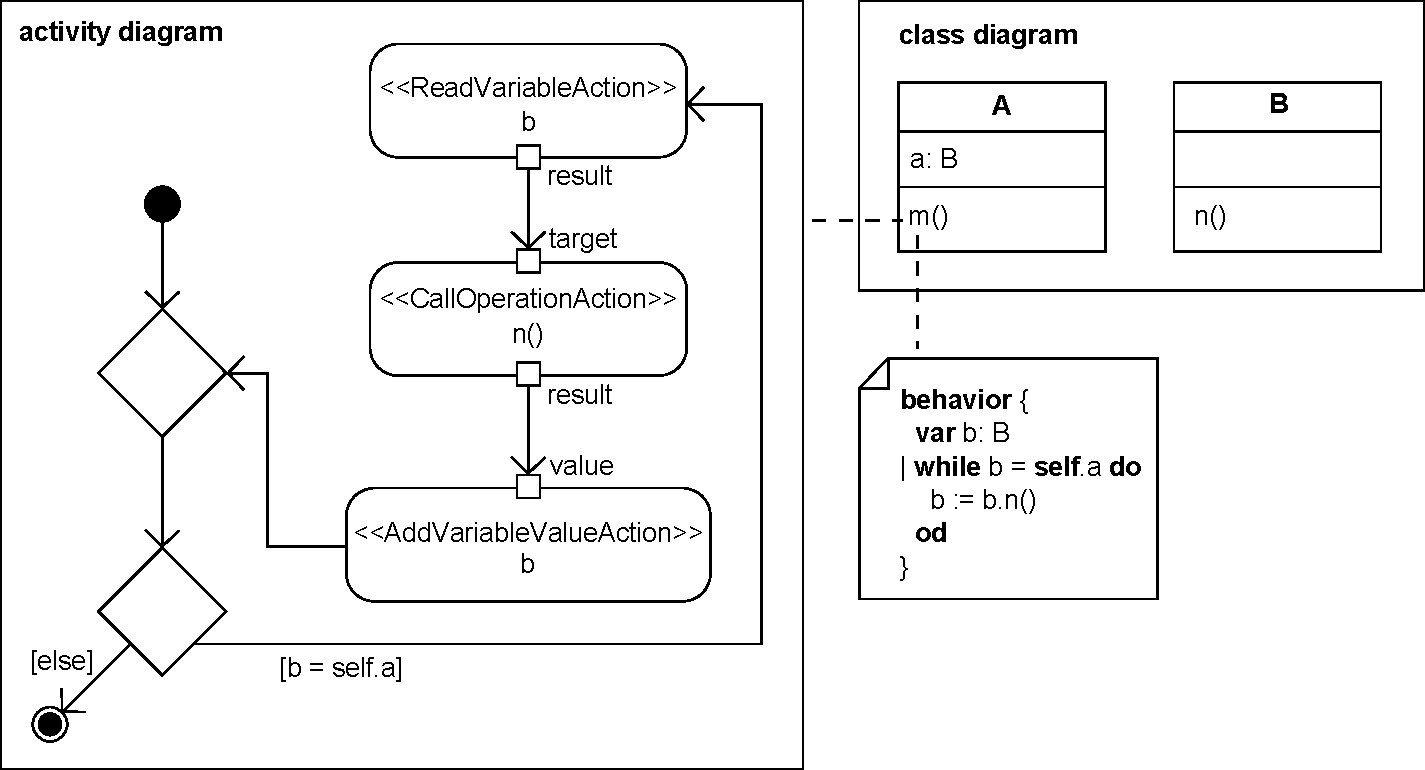
\includegraphics[scale=0.5]{grammars-and-metamodels/figs/diagram-comparison}
\caption{Two representations of the same behavior}
\label{fig:grammars-and-metamodels:UML-diagram-comparison}
\end{figure}

\Activities are one of the concepts offered by the \UML to specify behavior.
Some aspects of an \Activity can be visualized in an activity diagram.
The leftmost part of Figure~\ref{fig:grammars-and-metamodels:UML-diagram-comparison} shows an example of such a diagram.

An \Activity is a directed graph, whose nodes and edges are called \ActivityNodes and \ActivityEdges.
There are a number of different \ActivityNodes, such as \ControlNodes (depicted by diamonds) and \Actions (depicted by rounded rectangles), and two types of \ActivityEdges, namely \ControlFlows and \ObjectFlows.

The informal description of the semantics of Activities states that the order in which \Actions are executed is based on the flow of tokens.
There are two kinds of tokens: control tokens and object tokens.
\ControlFlows, which are depicted by arrows connecting \ActivityNodes, show how control tokens flow from one \ActivityNode to the other.
\ObjectFlows, which are depicted by arrows connecting \OutputPins and \InputPins, show how object tokens flow from one \Action producing an object to another \Action that uses this object.

The \ObjectFlows in Figure~\ref{fig:grammars-and-metamodels:UML-diagram-comparison} are depicted by the arrows connecting the small rectangles on the borders of the \Actions.
These small rectangles are the \InputPins and \OutputPins of those \Actions.


\subsection{Surface Languages}
\label{sub:grammars-and-metamodels:Prelim-SL}

Every model conforms to a metamodel, which defines the elements that play a role in the model.
If a model conforms to a certain metamodel, each element of the model is an instance of an element in that metamodel.
The \UML defines a number of diagrams, which can be used to depict certain parts of a model.
There are diagrams that depict the structure of a model, diagrams that depict the behavior of parts of the model, etc.
These diagrams offer a graphical representation for instances of elements in the metamodel.

In the context of the \UML, the term \emph{surface language} is used to refer to a concrete syntax that offers an alternative notation for these diagrams.
In our case, instead of a graphical representation, a textual representation is given for instances of elements of the metamodel.
Other names for surface languages related to \Activities and \Actions are \emph{surface action languages} and \emph{action languages}. 